\documentclass{minimal}
\usepackage{tikz}
\pagestyle{empty}

\begin{document}
\raggedright

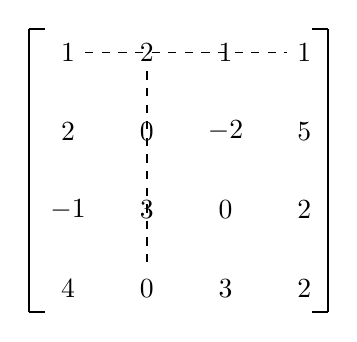
\begin{tikzpicture}[semithick]
  \draw [thick] (-0.5, -0.3) -- (-0.5, 3.3);
  \draw [thick] (-0.5, -0.3) -- (-0.3, -0.3);
  \draw [thick] (-0.5, 3.3)  -- (-0.3, 3.3);

  \node (a) at (0, 3) {$1$};
  \node (b) at (1, 3) {$2$};
  \node (c) at (2, 3) {$1$};
  \node (d) at (3, 3) {$1$};

  \node (e) at (0, 2) {$2$};
  \node (f) at (1, 2) {$0$};
  \node (g) at (2, 2) {$-2$};
  \node (h) at (3, 2) {$5$};

  \node (i) at (0, 1) {$-1$};
  \node (j) at (1, 1) {$3$};
  \node (k) at (2, 1) {$0$};
  \node (l) at (3, 1) {$2$};

  \node (m) at (0, 0) {$4$};
  \node (n) at (1, 0) {$0$};
  \node (o) at (2, 0) {$3$};
  \node (p) at (3, 0) {$2$};

  \draw [dashed] (a) -- (d);
  \draw [dashed] (b) -- (n);

  \draw [thick] (3.3, -0.3) -- (3.3, 3.3);
  \draw [thick] (3.3, -0.3) -- (3.1, -0.3);
  \draw [thick] (3.3, 3.3)  -- (3.1, 3.3);

\end{tikzpicture}

\vspace{1cm}


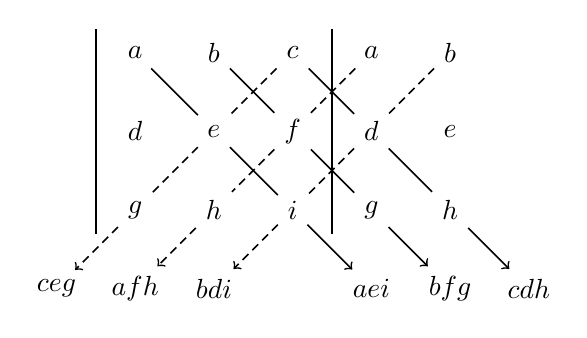
\begin{tikzpicture}[semithick]
  \draw [thick] (-0.5, -0.3) -- (-0.5, 2.3);

  \node (a) at (0, 2) {$a$};
  \node (b) at (1, 2) {$b$};
  \node (c) at (2, 2) {$c$};

  \node (d) at (0, 1) {$d$};
  \node (e) at (1, 1) {$e$};
  \node (f) at (2, 1) {$f$};

  \node (g) at (0, 0) {$g$};
  \node (h) at (1, 0) {$h$};
  \node (i) at (2, 0) {$i$};

  \draw [thick] (2.5, -0.3) -- (2.5, 2.3);

  \node (a2) at (3, 2) {$a$};
  \node (d2) at (3, 1) {$d$};
  \node (g2) at (3, 0) {$g$};

  \node (b2) at (4, 2) {$b$};
  \node (e2) at (4, 1) {$e$};
  \node (h2) at (4, 0) {$h$};

  \draw 
        (a) -- (e)   (e)  -- (i)
        (b) -- (f)   (f)  -- (g2)
        (c) -- (d2)  (d2) -- (h2);

  \draw [densely dashed]
        (b2) -- (d2)  (d2) -- (i)
        (a2) -- (f)   (f)  -- (h)
        (c) --  (e)   (e)  -- (g);
 
  \node (p1) at (3, -1) {$aei$};
  \node (p2) at (4, -1) {$bfg$};
  \node (p3) at (5, -1) {$cdh$};

  \node (s1) at (-1, -1) {$ceg$};
  \node (s2) at (0, -1) {$afh$};
  \node (s3) at (1, -1) {$bdi$};

  \draw [->] (i)  -- (p1);
  \draw [->] (g2) -- (p2);
  \draw [->] (h2) -- (p3);

  \draw [densely dashed, ->] (g) -- (s1);
  \draw [densely dashed, ->] (h) -- (s2);
  \draw [densely dashed, ->] (i) -- (s3);
\end{tikzpicture}

\vspace{1cm}

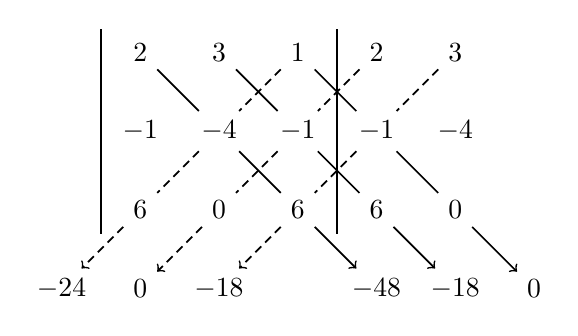
\begin{tikzpicture}[semithick]
  \draw [thick] (-0.5, -0.3) -- (-0.5, 2.3);

  \node (a1-1) at (0, 2) {$2$};
  \node (a1-2) at (1, 2) {$3$};
  \node (a1-3) at (2, 2) {$1$};

  \node (a2-1) at (0, 1) {$-1$};
  \node (a2-2) at (1, 1) {$-4$};
  \node (a2-3) at (2, 1) {$-1$};

  \node (a3-1) at (0, 0) {$6$};
  \node (a3-2) at (1, 0) {$0$};
  \node (a3-3) at (2, 0) {$6$};

  \draw [thick] (2.5, -0.3) -- (2.5, 2.3);

  \node (a1-4) at (3, 2) {$2$};
  \node (a2-4) at (3, 1) {$-1$};
  \node (a3-4) at (3, 0) {$6$};

  \node (a1-5) at (4, 2) {$3$};
  \node (a2-5) at (4, 1) {$-4$};
  \node (a3-5) at (4, 0) {$0$};

  \draw 
        (a1-1) -- (a2-2)  (a2-2) -- (a3-3)
        (a1-2) -- (a2-3)  (a2-3) -- (a3-4)
        (a1-3) -- (a2-4)  (a2-4) -- (a3-5);

  \draw [densely dashed]
        (a1-3) -- (a2-2)  (a2-2) -- (a3-1)
        (a1-4) -- (a2-3)  (a2-3) -- (a3-2)
        (a1-5) -- (a2-4)  (a2-4) -- (a3-3);
 
  \node (p1) at (3, -1) {$-48$};
  \node (p2) at (4, -1) {$-18$};
  \node (p3) at (5, -1) {$0$};

  \node (s1) at (-1, -1) {$-24$};
  \node (s2) at (0, -1) {$0$};
  \node (s3) at (1, -1) {$-18$};

  \draw [->] (a3-3) -- (p1);
  \draw [->] (a3-4) -- (p2);
  \draw [->] (a3-5) -- (p3);

  \draw [densely dashed, ->] (a3-1) -- (s1);
  \draw [densely dashed, ->] (a3-2) -- (s2);
  \draw [densely dashed, ->] (a3-3) -- (s3);
\end{tikzpicture}


\vspace{1cm}

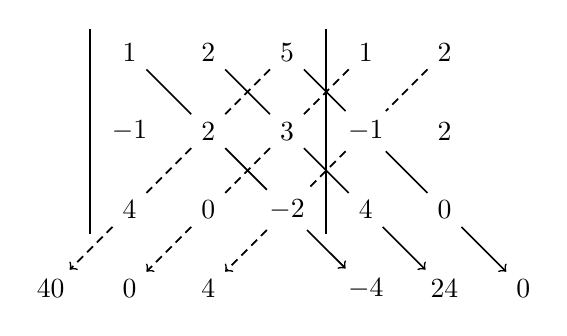
\begin{tikzpicture}[semithick]
  \draw [thick] (-0.5, -0.3) -- (-0.5, 2.3);

  \node (a1-1) at (0, 2) {$1$};
  \node (a1-2) at (1, 2) {$2$};
  \node (a1-3) at (2, 2) {$5$};

  \node (a2-1) at (0, 1) {$-1$};
  \node (a2-2) at (1, 1) {$2$};
  \node (a2-3) at (2, 1) {$3$};

  \node (a3-1) at (0, 0) {$4$};
  \node (a3-2) at (1, 0) {$0$};
  \node (a3-3) at (2, 0) {$-2$};

  \draw [thick] (2.5, -0.3) -- (2.5, 2.3);

  \node (a1-4) at (3, 2) {$1$};
  \node (a2-4) at (3, 1) {$-1$};
  \node (a3-4) at (3, 0) {$4$};

  \node (a1-5) at (4, 2) {$2$};
  \node (a2-5) at (4, 1) {$2$};
  \node (a3-5) at (4, 0) {$0$};

  \draw 
        (a1-1) -- (a2-2)  (a2-2) -- (a3-3)
        (a1-2) -- (a2-3)  (a2-3) -- (a3-4)
        (a1-3) -- (a2-4)  (a2-4) -- (a3-5);

  \draw [densely dashed]
        (a1-3) -- (a2-2)  (a2-2) -- (a3-1)
        (a1-4) -- (a2-3)  (a2-3) -- (a3-2)
        (a1-5) -- (a2-4)  (a2-4) -- (a3-3);
 
  \node (p1) at (3, -1) {$-4$};
  \node (p2) at (4, -1) {$24$};
  \node (p3) at (5, -1) {$0$};

  \node (s1) at (-1, -1) {$40$};
  \node (s2) at (0, -1) {$0$};
  \node (s3) at (1, -1) {$4$};

  \draw [->] (a3-3) -- (p1);
  \draw [->] (a3-4) -- (p2);
  \draw [->] (a3-5) -- (p3);

  \draw [densely dashed, ->] (a3-1) -- (s1);
  \draw [densely dashed, ->] (a3-2) -- (s2);
  \draw [densely dashed, ->] (a3-3) -- (s3);
\end{tikzpicture}

\vspace{1cm}

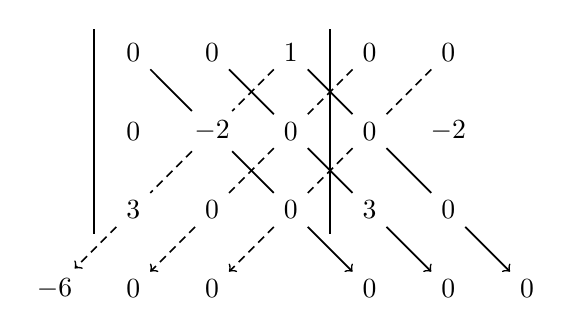
\begin{tikzpicture}[semithick]
  \draw [thick] (-0.5, -0.3) -- (-0.5, 2.3);

  \node (a1-1) at (0, 2) {$0$};
  \node (a1-2) at (1, 2) {$0$};
  \node (a1-3) at (2, 2) {$1$};

  \node (a2-1) at (0, 1) {$0$};
  \node (a2-2) at (1, 1) {$-2$};
  \node (a2-3) at (2, 1) {$0$};

  \node (a3-1) at (0, 0) {$3$};
  \node (a3-2) at (1, 0) {$0$};
  \node (a3-3) at (2, 0) {$0$};

  \draw [thick] (2.5, -0.3) -- (2.5, 2.3);

  \node (a1-4) at (3, 2) {$0$};
  \node (a2-4) at (3, 1) {$0$};
  \node (a3-4) at (3, 0) {$3$};

  \node (a1-5) at (4, 2) {$0$};
  \node (a2-5) at (4, 1) {$-2$};
  \node (a3-5) at (4, 0) {$0$};

  \draw 
        (a1-1) -- (a2-2)  (a2-2) -- (a3-3)
        (a1-2) -- (a2-3)  (a2-3) -- (a3-4)
        (a1-3) -- (a2-4)  (a2-4) -- (a3-5);

  \draw [densely dashed]
        (a1-3) -- (a2-2)  (a2-2) -- (a3-1)
        (a1-4) -- (a2-3)  (a2-3) -- (a3-2)
        (a1-5) -- (a2-4)  (a2-4) -- (a3-3);
 
  \node (p1) at (3, -1) {$0$};
  \node (p2) at (4, -1) {$0$};
  \node (p3) at (5, -1) {$0$};

  \node (s1) at (-1, -1) {$-6$};
  \node (s2) at (0, -1) {$0$};
  \node (s3) at (1, -1) {$0$};

  \draw [->] (a3-3) -- (p1);
  \draw [->] (a3-4) -- (p2);
  \draw [->] (a3-5) -- (p3);

  \draw [densely dashed, ->] (a3-1) -- (s1);
  \draw [densely dashed, ->] (a3-2) -- (s2);
  \draw [densely dashed, ->] (a3-3) -- (s3);
\end{tikzpicture}

\vspace{1cm}

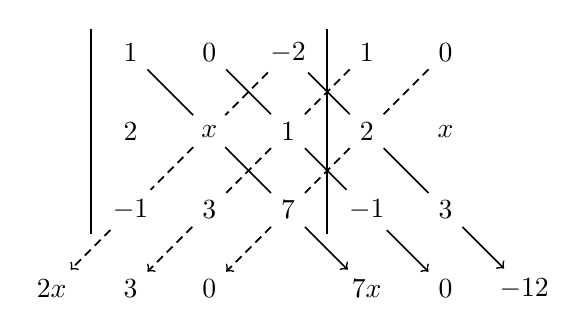
\begin{tikzpicture}[semithick]
  \draw [thick] (-0.5, -0.3) -- (-0.5, 2.3);

  \node (a1-1) at (0, 2) {$1$};
  \node (a1-2) at (1, 2) {$0$};
  \node (a1-3) at (2, 2) {$-2$};

  \node (a2-1) at (0, 1) {$2$};
  \node (a2-2) at (1, 1) {$x$};
  \node (a2-3) at (2, 1) {$1$};

  \node (a3-1) at (0, 0) {$-1$};
  \node (a3-2) at (1, 0) {$3$};
  \node (a3-3) at (2, 0) {$7$};

  \draw [thick] (2.5, -0.3) -- (2.5, 2.3);

  \node (a1-4) at (3, 2) {$1$};
  \node (a2-4) at (3, 1) {$2$};
  \node (a3-4) at (3, 0) {$-1$};

  \node (a1-5) at (4, 2) {$0$};
  \node (a2-5) at (4, 1) {$x$};
  \node (a3-5) at (4, 0) {$3$};

  \draw 
        (a1-1) -- (a2-2)  (a2-2) -- (a3-3)
        (a1-2) -- (a2-3)  (a2-3) -- (a3-4)
        (a1-3) -- (a2-4)  (a2-4) -- (a3-5);

  \draw [densely dashed]
        (a1-3) -- (a2-2)  (a2-2) -- (a3-1)
        (a1-4) -- (a2-3)  (a2-3) -- (a3-2)
        (a1-5) -- (a2-4)  (a2-4) -- (a3-3);
 
  \node (p1) at (3, -1) {$7x$};
  \node (p2) at (4, -1) {$0$};
  \node (p3) at (5, -1) {$-12$};

  \node (s1) at (-1, -1) {$2x$};
  \node (s2) at (0, -1) {$3$};
  \node (s3) at (1, -1) {$0$};

  \draw [->] (a3-3) -- (p1);
  \draw [->] (a3-4) -- (p2);
  \draw [->] (a3-5) -- (p3);

  \draw [densely dashed, ->] (a3-1) -- (s1);
  \draw [densely dashed, ->] (a3-2) -- (s2);
  \draw [densely dashed, ->] (a3-3) -- (s3);
\end{tikzpicture}

\vspace{1cm}

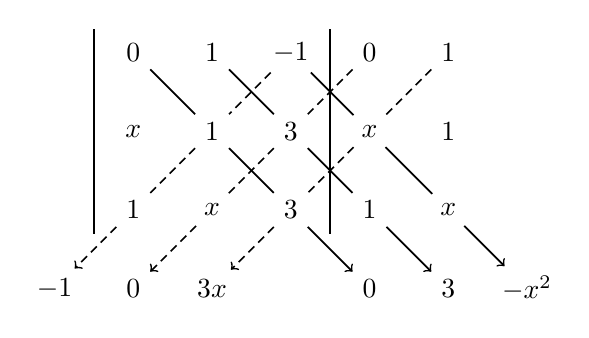
\begin{tikzpicture}[semithick]
  \draw [thick] (-0.5, -0.3) -- (-0.5, 2.3);

  \node (a1-1) at (0, 2) {$0$};
  \node (a1-2) at (1, 2) {$1$};
  \node (a1-3) at (2, 2) {$-1$};

  \node (a2-1) at (0, 1) {$x$};
  \node (a2-2) at (1, 1) {$1$};
  \node (a2-3) at (2, 1) {$3$};

  \node (a3-1) at (0, 0) {$1$};
  \node (a3-2) at (1, 0) {$x$};
  \node (a3-3) at (2, 0) {$3$};

  \draw [thick] (2.5, -0.3) -- (2.5, 2.3);

  \node (a1-4) at (3, 2) {$0$};
  \node (a2-4) at (3, 1) {$x$};
  \node (a3-4) at (3, 0) {$1$};

  \node (a1-5) at (4, 2) {$1$};
  \node (a2-5) at (4, 1) {$1$};
  \node (a3-5) at (4, 0) {$x$};

  \draw 
        (a1-1) -- (a2-2)  (a2-2) -- (a3-3)
        (a1-2) -- (a2-3)  (a2-3) -- (a3-4)
        (a1-3) -- (a2-4)  (a2-4) -- (a3-5);

  \draw [densely dashed]
        (a1-3) -- (a2-2)  (a2-2) -- (a3-1)
        (a1-4) -- (a2-3)  (a2-3) -- (a3-2)
        (a1-5) -- (a2-4)  (a2-4) -- (a3-3);
 
  \node (p1) at (3, -1) {$0$};
  \node (p2) at (4, -1) {$3$};
  \node (p3) at (5, -1) {$-x^2$};

  \node (s1) at (-1, -1) {$-1$};
  \node (s2) at (0, -1) {$0$};
  \node (s3) at (1, -1) {$3x$};

  \draw [->] (a3-3) -- (p1);
  \draw [->] (a3-4) -- (p2);
  \draw [->] (a3-5) -- (p3);

  \draw [densely dashed, ->] (a3-1) -- (s1);
  \draw [densely dashed, ->] (a3-2) -- (s2);
  \draw [densely dashed, ->] (a3-3) -- (s3);
\end{tikzpicture}

\vspace{1cm}

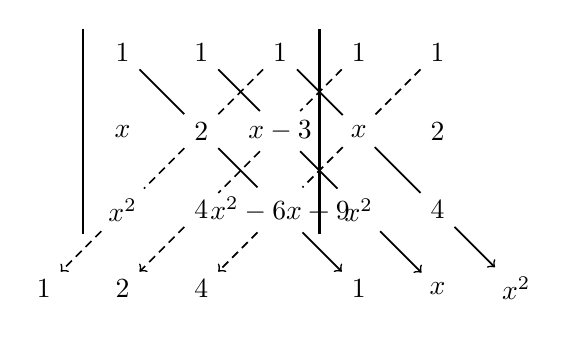
\begin{tikzpicture}[semithick]
  \draw [thick] (-0.5, -0.3) -- (-0.5, 2.3);

  \node (a1-1) at (0, 2) {$1$};
  \node (a1-2) at (1, 2) {$1$};
  \node (a1-3) at (2, 2) {$1$};

  \node (a2-1) at (0, 1) {$x$};
  \node (a2-2) at (1, 1) {$2$};
  \node (a2-3) at (2, 1) {$x-3$};

  \node (a3-1) at (0, 0) {$x^2$};
  \node (a3-2) at (1, 0) {$4$};
  \node (a3-3) at (2, 0) {$x^2-6x+9$};

  \draw [thick] (2.5, -0.3) -- (2.5, 2.3);

  \node (a1-4) at (3, 2) {$1$};
  \node (a2-4) at (3, 1) {$x$};
  \node (a3-4) at (3, 0) {$x^2$};

  \node (a1-5) at (4, 2) {$1$};
  \node (a2-5) at (4, 1) {$2$};
  \node (a3-5) at (4, 0) {$4$};

  \draw 
        (a1-1) -- (a2-2)  (a2-2) -- (a3-3)
        (a1-2) -- (a2-3)  (a2-3) -- (a3-4)
        (a1-3) -- (a2-4)  (a2-4) -- (a3-5);

  \draw [densely dashed]
        (a1-3) -- (a2-2)  (a2-2) -- (a3-1)
        (a1-4) -- (a2-3)  (a2-3) -- (a3-2)
        (a1-5) -- (a2-4)  (a2-4) -- (a3-3);
 
  \node (p1) at (3, -1) {$1$};
  \node (p2) at (4, -1) {$x$};
  \node (p3) at (5, -1) {$x^2$};

  \node (s1) at (-1, -1) {$1$};
  \node (s2) at (0, -1) {$2$};
  \node (s3) at (1, -1) {$4$};

  \draw [->] (a3-3) -- (p1);
  \draw [->] (a3-4) -- (p2);
  \draw [->] (a3-5) -- (p3);

  \draw [densely dashed, ->] (a3-1) -- (s1);
  \draw [densely dashed, ->] (a3-2) -- (s2);
  \draw [densely dashed, ->] (a3-3) -- (s3);
\end{tikzpicture}

\vspace{1cm}

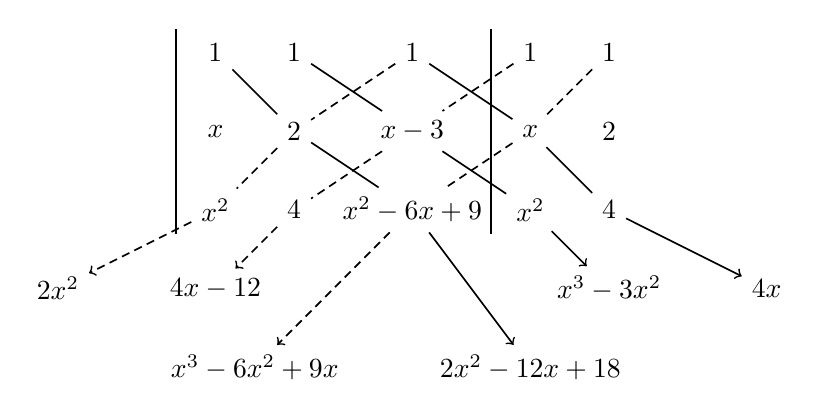
\begin{tikzpicture}[semithick]
  \draw [thick] (-0.5, -0.3) -- (-0.5, 2.3);

  \node (a) at (0, 2) {$1$};
  \node (b) at (1, 2) {$1$};
  \node (c) at (2.5, 2) {$1$};

  \node (d) at (0, 1) {$x$};
  \node (e) at (1, 1) {$2$};
  \node (f) at (2.5, 1) {$x-3$};

  \node (g) at (0, 0) {$x^2$};
  \node (h) at (1, 0) {$4$};
  \node (i) at (2.5, 0) {$x^2-6x+9$};

  \draw [thick] (3.5, -0.3) -- (3.5, 2.3);

  \node (a2) at (4, 2) {$1$};
  \node (d2) at (4, 1) {$x$};
  \node (g2) at (4, 0) {$x^2$};

  \node (b2) at (5, 2) {$1$};
  \node (e2) at (5, 1) {$2$};
  \node (h2) at (5, 0) {$4$};

  \draw 
        (a) -- (e)   (e)  -- (i)
        (b) -- (f)   (f)  -- (g2)
        (c) -- (d2)  (d2) -- (h2);

  \draw [densely dashed]
        (b2) -- (d2)  (d2) -- (i)
        (a2) -- (f)   (f)  -- (h)
        (c) --  (e)   (e)  -- (g);
 
  \node (p1) at (4, -2) {$2x^2-12x+18$};
  \node (p2) at (5, -1) {$x^3-3x^2$};
  \node (p3) at (7, -1) {$4x$};

  \node (s1) at (-2, -1) {$2x^2$};
  \node (s2) at (0, -1) {$4x-12$};
  \node (s3) at (0.5, -2) {$x^3-6x^2+9x$};

  \draw [->] (i)  -- (p1);
  \draw [->] (g2) -- (p2);
  \draw [->] (h2) -- (p3);

  \draw [densely dashed, ->] (g) -- (s1);
  \draw [densely dashed, ->] (h) -- (s2);
  \draw [densely dashed, ->] (i) -- (s3);
\end{tikzpicture}

\end{document}
